\documentclass[a4paper]{article}
\usepackage[utf8]{inputenc}
\usepackage[margin=50pt]{geometry}
\usepackage{tabularx}
\usepackage{tabulary}
\usepackage{graphicx}
\usepackage{xcolor}
\usepackage{hyperref}

\hypersetup{
    colorlinks=true,
    linkcolor=blue,
}


\title{Ingegneria del Software T}
\author{
    Luca Bartolomei 
    \texttt{0000825005}
    \\
    Luigi Di Nuzzo
    \texttt{0000824873}
    \\
    Filippo Veronesi
    \texttt{0000832244}
}

\date{Marzo 2020}

\begin{document}

\maketitle

\tableofcontents

\newpage

\section{Abstract}

Il progetto riguarda la creazione di un applicativo software gestionale per prevendite elettroniche.\\
Abbiamo pensato il software per un gruppo di amici che organizzano feste, con obiettivi cardine l'abbattimento di costi, l'ottimizzazione dell'entrata dei partecipanti all'evento e una semplificazione dei conti di bilancio.\\
L'idea di fondo è di utilizzare, come sostitutivo alla prevendita cartacea, un codice QR in grado di far entrare il cliente dopo relativo check all'entrata.\\
Il risparmio economico ottenuto è ovviamente importante in confronto alla vendita tradizionale. Tuttavia bisogna tenere in conto dei problemi tecnologici che si possono verificare durante la vendita e l'entrata: problemi di connessione Internet, incompatibilità dei dispositivi dei clienti, training del personale addetto alle entrate, eccetera.\\
Viene gestito oltre alle prevendite e relatvi clienti, anche l'organizzazione e i vari membri dell'organizzazione, con divisione dei ruoli.\\
Per facilitare i conti di bilancio è disponibile una sezione in cui è possibile ricavare statistiche sull'andamento dell'evento.

\newpage

\section{Analisi dei requisiti}

\subsection{Requisiti del sistema}

\begin{itemize}
	
	\item \textbf{REQUISITI FUNZIONALI}
		
	\item \hypertarget{R1F}{R1F} - Il software prevede la possibilità di gestire più staff.
	
	%-Requisiti di sicurezza
	
	%--Requisiti di identificazione
	\item \hypertarget{R2F}{R2F} - Gli utenti devono essere identificati tramite username.
	
	%--Requisito di autenticazione
	\item \hypertarget{R3F}{R3F} - Gli utenti sono autenticati tramite credenziali di username e password.
	\item \hypertarget{R4F}{R4F} - L'accesso ad uno staff, da parte di un utente, avviene tramite codice di accesso.	

	%Funzionale/non funzionale
	\item \hypertarget{R5F}{R5F} - La registrazione di utenti è a carico dell'amministratore di sistema.
	\item \hypertarget{R6F}{R6F} - Possibilità di cambiare la password personale dell'utente.
		
	%--Requisiti di Autorizzazione
	\item \hypertarget{R7F}{R7F} - Ogni membro di uno staff può ricoprire dei ruoli: cassiere, PR, amministratore.	
	\item \hypertarget{R8F}{R8F} - Il ruolo di cassiere riguarda la timbratura di prevendite all'ingresso di un evento.
	\item \hypertarget{R9F}{R9F} - Il ruolo di PR riguarda la vendita di prevendite a clienti.
	\item \hypertarget{R10F}{R10F} - Il ruolo di amministratore riguarda la gestione dei membri, degli eventi, delle tipologie di prevendita di un evento e della visualizzazione di tutte statistiche.
	
	%--Requisiti di scoperta alle intrusioni
	%\item \hypertarget{R11F}{R11F} - Utilizzo di log per monitorare operazioni critiche.

	%--Requisiti di riservatezza
	\item \hypertarget{R12F}{R12F} - Le password devono essere salvate in modo sicuro.
	
	%Non vuol dire cifrato! Basta un controllo agli accessi.
	%Se salvi in DB ricorda di indicizzare.
	%\item Il log deve essere salvato in modo abbastanza sicuro.
	
	%--------------------
	
	%Accesso e creazione di uno staff
	\item \hypertarget{R13F}{R13F} - Ogni utente registrato nel gestionale può diventare membro di uno o più staff. 
	
	\item \hypertarget{R14F}{R14F} - Quando un utente crea uno staff ne diventa membro e amministratore.
	
	%Timbratura (Cassiere)
	\item \hypertarget{R15F}{R15F} - La timbratura di una prevendita valida permette al cliente di entrare all'evento, ovviamente lo staff potrà effettuare ulteriori controlli non previsti dal sistema e decidere di far entrare un cliente.
	
	\item \hypertarget{R16F}{R16F} - Il documento digitale consegnato al cliente sarà utilizzato dal cassiere all'ingresso timbrare la prevedita elettronica.
	
	
	%Non viene specificata la modalità di consegna: URL, file immagine file testo etc.
	\item \hypertarget{R17F}{R17F} - La vendita di una prevendita elettronica consiste nella consegna al cliente di un documento digitale di qualche forma, associato alla prevendita elettronica venduta.

	
	%Gestione staff (Amministratore)
	\item \hypertarget{R18F/NF}{R18F/NF} - Un amministratore può concedere/revocare i ruoli a qualsiasi membro dello staff. Unico vincolo è che rimanga almeno un amministratore.
	\item \hypertarget{R19F}{R19F} - Possibilità di cambiare il codice di accesso dello staff da parte di un amministratore.
	   
	\item \hypertarget{R20F}{R20F} - Per gestione degli eventi di uno staff si intende la possibilità di vedere gli staff di un evento, di creane uno nuovo e di poter modificare un evento dello staff.
		
	\item \hypertarget{R21F}{R21F} - La gestione delle tipologie di prevedita di un evento indica l'aggiunta, la modifica e la rimozione delle tipologie di prevendita.
	
	%Definizioni
	%-Eventi
	\item \hypertarget{R22F}{R22F} - Un evento è composto da un nome, una descrizione, un periodo temporale di svolgimento e un luogo. 
	\item \hypertarget{R23F}{R23F} - Un evento può essere annullato, anche se ci sono prevendite vendute.
	
	%Tipologia Prevendita
	\item \hypertarget{R24F}{R24F} - Una tipologia di prevendita serve ad associare alla prevendita un prezzo, una descrizione e un periodo di vendita a tutte le prevendite con la stessa tipologia.

	%-Prevendite
	\item \hypertarget{R25F}{R25F} - Una prevendita può essere annullata e/o rimborsata. 
	
	%-Statistiche
	\item \hypertarget{R26F}{R26F} - Le statistiche di un membro sono suddivise per ruolo coperto all'interno dello staff: cassiere o PR.
	
	\item \hypertarget{R27F}{R27F} - Lo sblocco dell'utente è a carico dell'amministratore di sistema.
	
	\item \hypertarget{R28F}{R28F} - Ogni prevedita è nominativa.
	
	%Si deduce dalla precedente
	%\item Il ruolo di amministratore non prevede statistiche personali.
		
    \item \textbf{REQUISITI NON FUNZIONALI}
	
	%Se si verifica attacco freezing dell'account cambiare username.
	\item \hypertarget{R1NF}{R1NF} - Il blocco dell'account deve avvenire dopo 3 tentativi.
	
	\item \hypertarget{R2NF}{R2NF} - La password degli utenti deve essere lunga almeno 8 caratteri.
	\item \hypertarget{R3NF}{R3NF} - Il codice di accesso allo staff deve essere lungo almeno 4 caratteri.
	\item \hypertarget{R4NF}{R4NF} - Ogni utente registrato può creare al massimo uno staff.
	\item \hypertarget{R5NF}{R5NF} - Requisito fondamentale è il basso costo del prodotto software.
	\item \hypertarget{R6NF}{R6NF} - Utilizzare uno o più metodi per velocizzare l'autenticazione dell'utente.
	\item \hypertarget{R7NF}{R7NF} - I membri non amministratori possono vedere solo le statistiche personali.	
	\item \hypertarget{R8NF}{R8NF} - I membri non amministratori possono solo vedere le tipologie di prevendite associate ad un evento.
	\item \hypertarget{R9NF}{R9NF} - I membri non amministratori possono solo vedere gli eventi dello staff.
	\item \hypertarget{R10NF}{R10NF} - Il periodo di vendita delle prevendite deve essere antecedente il periodo dell'evento.
	\item \hypertarget{R11NF}{R11NF} - Una prevendita annullata e/o rimborsata rimane tale.
	\item \hypertarget{R12NF}{R12NF} - Un evento annullato rimane tale.
	\item \hypertarget{R13NF}{R13NF} - Si prevedono più forme di consegna del documento digitale, per affrontare le eterogeneità.
	\item \hypertarget{R14NF}{R14NF} - La password fornita dall'amministratore di sistema a tempo di registrazione va cambiata immediatamente dopo il login.
	
	%Devo contare i tentativi falliti nel db: nella sessione potrei cancellare i cookie.
	\item \hypertarget{R15NF}{R15NF} - Bloccare l'account utente dopo troppi tentativi di accesso e notificarlo nei log.
	
	\item \hypertarget{R16NF}{R16NF} - Ogni ruolo è indipendente.
	\item \hypertarget{R17NF}{R17NF} - Ogni staff gestito dal software è indipendente.
	
	%Utilizzo https per la cifratura
	\item \hypertarget{R18NF}{R18NF} - Si richiede una comunicazione sicura.
	
	%Sistema locale senza server remoto tramite server locale + wifi
	\item \hypertarget{R19NF}{R19NF} - Si richiedono procedure manuali o automatiche per cercare di garantire la disponibilità del servizio.
	
	%Codice della prevendita
	%Prevendita nominativa
	\item \hypertarget{R20NF}{R20NF} - Si richiedono metodi per evitare la contraffazione delle prevendite.
	
	%Log
	%\item \hypertarget{R21NF}{R21NF} - Prevedere livelli di log per aiutare l'analisi da parte dell'amministratore di sistema.
	
	%Prevendita
	\item \hypertarget{R22NF}{R22NF} - Ogni prevendita venduta è associata ad una sola tipologia di prevendita.
	\item \hypertarget{R23NF}{R23NF} - La tipologia di prevendita associata non è modificabile.
	
	%Tipologia prevendita
	\item \hypertarget{R25NF}{R25NF} - Il prezzo di una tipologia di prevendita è modificabile solo se non sono state vendute prevendite con quella determinata tipologia.
	
	%--Requisiti di non-ripudiabilità
	\item \hypertarget{R26NF}{R26NF} - Quando un PR vende una prevendita, essa viene associata ad esso.
	\item \hypertarget{R27NF}{R27NF} - Quando un Cassiere timbra una prevendita, essa viene associata ad esso.
	
	%Vendita (PR)
	\item \hypertarget{R6NF}{R28NF} - Prima della vendita il cliente sceglierà una tipologia di prevendita associata all'evento a cui vuole partecipare.
	
	\item \hypertarget{R29NF}{R29NF} - La timbratura può essere fatta solo una volta.
	
	
\end{itemize}

\newpage

\subsection{Analisi del dominio}

\subsubsection{Glossario}

\begin{table}[ht!]
  \begin{center}
    \begin{tabulary}{1\textwidth}{|c|C|C|}
        \hline
        \textbf{Voce} & \textbf{Definizione} & \textbf{Sinonimi}\\
        \hline
        \hline
		Amministratore di sistema & Utente con privilegi di sistema aggiuntivi. & \\
		\hline
		Privilegio di sistema & Autorizzazione intrinseca concessa ad un amministratore di sistema che riguarda la gestione del software stesso. Non riguarda gli staff. & \\
		\hline
        Staff & Gruppo di utenti con lo scopo di organizzare eventi. & Ente organizzatore \\
        \hline
        Utente & Persona registrata nel software gestione. & \\
        \hline
		Cliente & Persona che vuole partecipare ad un evento di uno staff & \\
		\hline
        Membro & Utente che è iscritto ad uno staff. & Organizzatore \\
        \hline
		PR & Membro di uno staff che si occupa della vendita di prevendite & \\
		\hline
		Cassiere & Membro di uno staff che si occupa dell'entrata dei clienti ad un evento & \\
		\hline
		Amministratore & Membro di uno staff che si occupa della gestione dello staff steso & \\
		\hline
        Ruolo & Autorizzazione che ha il membro all'interno dello staff & Autorizzazione \\
        \hline
        Evento & Avvenimento registrato dallo staff, per il quale è possibile vendere prevendite e registrare ingressi & Festa \\
        \hline
        Tipologia Prevendita & Modello associato ad un evento, la quale da le caratteristiche di prezzo e descrizione alla prevendita venduta & Tipo Prevendita \\
        \hline
        Prevendita & Biglietto venduto anticipatamente, che consente l'entrata all'evento pagato & Ticket, Prevendita Elettronica \\
        \hline
		Statistiche & Informazioni di carattere gestionale, riguardo ad un evento o a un membro dello staff & \\
		\hline
		Documento digitale & Si tratta di una risorsa digitale, reperibile dal cliente, che serve a identificare una prevendita venduta & \\
		\hline
		Log & Registro dove vengono salvate informazioni per risalire ad operazioni critiche svolte. Composto da una serie di voci & Registro \\
		\hline
		Voce di log & Si tratta di una riga del log. & Record del log\\
		\hline
		Operazione & Comando richiesto al software gestionale da parte di un utente & \\
		\hline
		Login & Operazione per identificare un utente & Accesso utente \\
		\hline
		Timbratura & Operazione svolta da un cassiere svolta per validare una prevendita di un cliente & Convalida della prevendita \\
		\hline
		Credenziali & Coppia di valori username e password utilizzata per l'autenticazione dell'utente & \\
		\hline
		Username & Stringa di caratteri alfanumerici. Serve a identificare l'utente & \\
		\hline
		Password & String di caratteri alfanumerici. Può contenere caratteri speciali. & \\
		\hline
		Periodo di vendita & Periodo temporale in cui la prevendita è vendibile ai clienti & \\
		\hline
    \end{tabulary}
  \end{center}
\end{table}

\newpage

\subsection{Analisi dei requisiti}
\subsubsection{Casi d'uso}

%Specificare i casi d'uso?
%Gestione utente: Sblocco utente, Registrazione utente
%Gestione Log: leggi Log, aggiungi log, cancella log
%Gestione vendita prevendita: aggiungi prevendita, annulla prevendita
%Gestione entrata: timbra entrata, leggi prevendita,
%Gestione eventi: aggiungi evento, modifica evento, annulla evento
%Gestione tipologie prevendite: aggiungi tipologia prevendita, modifica tipologia prevendita, elimina tipologia prevendita.

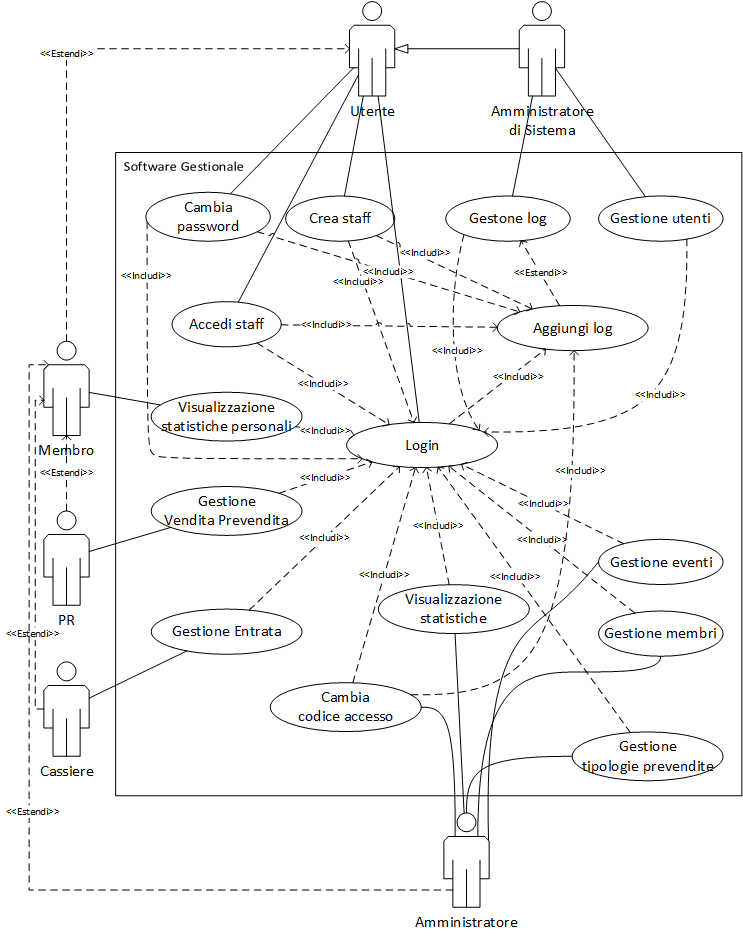
\includegraphics[scale=0.9]{use_cases.png}

L'utilizzo del login (frecce \textcolor{orange}{arancioni}) è necessario per tutti i servizi forniti agli attori.
Tutte le funzioni che abbiamo ritenute critiche utilizzano il caso d'uso "Aggiungi log" (frecce \textcolor{blue}{blu}).
Con le frecce \textcolor{violet}{viola} abbiamo voluto evidenziare la maggior parte degli scenari che estendono la gestione degli utenti o dello staff.\\
Abbiamo differenziato i casi d'uso delle statistiche perché si tratta di concetti diversi.    





\newpage

\subsubsection{Scenari}

%Login

\begin{center}
\begin{tabularx}{1\textwidth}{|l|X|}
    \hline
	\textbf{Titolo} & Login \\
	\hline
	\textbf{Descrizione} & Autenticazione nel software gestionale \\
	\hline
	\textbf{Attori} & Utente \\
	\hline
	\textbf{Relazioni} & Cambia Password \\
	\hline
	\textbf{Precondizioni} & L'utente deve essere registato nel sistema \\
	\hline
	\textbf{Postcondizioni} & L'utente è autenticato nel sistema \\
	\hline
	\textbf{Scenario principale} & 1. Impostazione di una schermata per l'inserimento di username e password. \\
								 & 2. L'utente inserisce i dati del proprio account. \\
								 & 3. L'utente esegue l'operazione. \\
								 & 4. Il sistema verifica le credenziali. \\
								 & 5. Dopo l'autenticazione viene mostrata una schermata principale.\\
	\hline
	\textbf{Scenari alternativi} & A) L'utente sbaglia credenziali: \\
								 & \quad 1. Notifica all'utente.\\
								 & \quad 2. Ritorno alla schermata di login.\\
								 & B) L'utente ha sbagliato troppe volte le credenziali: \\
								 & \quad 1. Blocco dell'account.\\
								 & \quad 2. Notifica all'utente.\\
								 & \quad 3. Ritorno alla schermata di login.\\
								 & C) L'utente ha la password di default impostata dall'amministratore di sistema:\\
								 & \quad 1. Passaggio al cambio password.\\
								 & D) L'utente ha l'account bloccato:\\
								 & \quad 1. Notifica all'utente.\\
								 & \quad 2. Ritorno alla schermata di login.\\
								 & E) L'utente è gia autenticato:\\
								 & \quad 1. Mostro la schermata principale.\\
	\hline
	\textbf{Requisiti non funzionali} & \hyperlink{R1NF}{R1NF}, \hyperlink{R2NF}{R2NF}, \hyperlink{R6NF}{R6NF}, \hyperlink{R15NF}{R15NF}, \hyperlink{R16NF}{R16NF} \\
	\hline
	\textbf{Punti aperti} & \\
	\hline
\end{tabularx}
\end{center}
  
%Gestione utenti

\begin{center}
\begin{tabularx}{1\textwidth}{|l|X|}
    \hline
	\textbf{Titolo} & Gestione utenti \\
	\hline
	\textbf{Descrizione} & Gestione degli utenti presenti nel software gestionale \\
	\hline
	\textbf{Attori} & Utente \\
	\hline
	\textbf{Relazioni} & Login, Cambia password, Accedi staff, Crea staff, Gestione log, Registrazione utente, Sblocco utente \\
	\hline
	\textbf{Precondizioni} &  \\
	\hline
	\textbf{Postcondizioni} &  \\
	\hline
	\textbf{Scenario principale} & 1. Viene mostrata una schermata con le azioni possibili:\\
								 & \quad a. Cambia Password.\\
								 & \quad b. Accedi staff.\\
								 & \quad c. Crea staff.\\
								 & 1b. Se l'utente è anche amministratore di sistema, vengono aggiunte delle scelte:\\
								 & \quad d. Gestione log.\\
								 & \quad e. Registrazione utente.\\
								 & \quad f. Sblocco utente.\\
								 & 2. L'utente sceglie l'operazione desiderata.\\
								 & 3. Il sistema cambia vista a seconda della scelta.\\
	\hline
	\textbf{Scenari alternativi} & A) L'utente non è autenticato: \\
								 & \quad 1. Notifica all'utente.\\
								 & \quad 2. Passaggio al login.\\
	\hline
	\textbf{Requisiti non funzionali} & \\
	\hline
	\textbf{Punti aperti} & \\
	\hline
\end{tabularx}
\end{center}

%Qui metto i casi d'uso sotto gestione utente------------------------------------------

%Sblocco utente

\begin{center}
\begin{tabularx}{1\textwidth}{|l|X|}
    \hline
	\textbf{Titolo} & Sblocco utente \\
	\hline
	\textbf{Descrizione} & Caso in cui un utente è bloccato e chiede aiuto all'amministratore di sistema. \\
	\hline
	\textbf{Attori} & Amministratore di sistema, Utente \\
	\hline
	\textbf{Relazioni} & Gestione utente \\
	\hline
	\textbf{Precondizioni} &  \\
	\hline
	\textbf{Postcondizioni} &  \\
	\hline
	\textbf{Scenario principale} & 1. L'amministratore si informa riguardo l'utente.\\
								 & 2. L'utente si spiega di quanto accaduto con l'amministratore.\\
								 & 3. Se decide di sbloccarlo allora inserisce i dati nell'apposita vista.\\
								 & 4. L'amministratore esegue l'operazione e l'utente viene sbloccato.\\
	\hline
	\textbf{Scenari alternativi} & \\
	\hline
	\textbf{Requisiti non funzionali} & \\
	\hline
	\textbf{Punti aperti} & \\
	\hline
\end{tabularx}
\end{center}

%Registrazione utente

\begin{center}
\begin{tabularx}{1\textwidth}{|l|X|}
    \hline
	\textbf{Titolo} & Registrazione utente \\
	\hline
	\textbf{Descrizione} & Una persona ha richiesto l'accesso al sistema gestionale e l'amministratore vuole registrarlo. \\
	\hline
	\textbf{Attori} & Amministratore di sistema, Utente \\
	\hline
	\textbf{Relazioni} & Gestione utente \\
	\hline
	\textbf{Precondizioni} &  \\
	\hline
	\textbf{Postcondizioni} &  \\
	\hline
	\textbf{Scenario principale} & 1. L'amministratore si informa riguardo l'utente, chiedendo informazioni per la registrazione.\\
								 & 2. L'utente fornisce i dati all'amministratore.\\
								 & 3. L'amministratore sceglie username e password iniziale per l'utente, utilizzando criteri di sicurezza.\\
	\hline
	\textbf{Scenari alternativi} & A) Dati dell'utente da registrare in conflitto o non validi: \\
								 & \quad 1. Notifica all'amministratore.\\
								 & \quad 2. L'amministratore cerca di correggere i dati.\\
								 & \quad 3. L'amministratore ripete l'operazione.\\
	\hline
	\textbf{Requisiti non funzionali} & \hyperlink{R2NF}{R2NF} \\
	\hline
	\textbf{Punti aperti} & \\
	\hline
\end{tabularx}
\end{center}

% Gestione log
%Forse da dividere in aggiungi log, leggi log e cancella log.

\begin{center}
\begin{tabularx}{1\textwidth}{|l|X|}
    \hline
	\textbf{Titolo} & Gestione log \\
	\hline
	\textbf{Descrizione} & Gestione del log del software gestionale \\
	\hline
	\textbf{Attori} & Amministratore di sistema \\
	\hline
	\textbf{Relazioni} & Gestione utente \\
	\hline
	\textbf{Precondizioni} &  \\
	\hline
	\textbf{Postcondizioni} &  \\
	\hline
	\textbf{Scenario principale} & 1. L'amministratore di sistema sceglie una funzione: \\
								 & \quad a. Aggiungi log \\
								 & \quad b. Leggi log \\
								 & \quad c. Cancella log \\
								 & 2. L'amministratore di sistema esegue l'operazione.\\
								 & 3. Ritorno alla schermata precedente.\\
	\hline
	\textbf{Scenari alternativi} & \\
	\hline
	\textbf{Requisiti non funzionali} & \\
	\hline
	\textbf{Punti aperti} & \\
	\hline
\end{tabularx}
\end{center}


%Aggiungi log
%Non so se mettere la relazione con login.

% \begin{center}
% \begin{tabularx}{1\textwidth}{l|X}
% \textbf{Titolo} & Aggiungi log \\
% \hline
% \textbf{Descrizione} & Aggiunta di una voce di log nel sistema gestionale \\
% \hline
% \textbf{Attori} & Amministratore di sistema \\
% \hline
% \textbf{Relazioni} & Gestione log \\
% \hline
% \textbf{Precondizioni} &  \\
% \hline
% \textbf{Postcondizioni} &  \\
% \hline
% \textbf{Scenario principale} & 1. Il sistema mostra una vista per l'inserimento della voce del log.\\
% & 2. L'amministratore di sistema aggiunge le informazioni.\\
% & 3. L'amministratore esegue l'operazione.\\
% & 4. Ritorno alla schermata precedente.\\
% \hline
% \textbf{Scenari alternativi} & A) L'utente non è autenticato: \\
% & \quad 1. Notifica all'utente.\\
% & \quad 2. Passaggio al login.\\
% & B) L'utente non è amministratore di sistema:\\
% & \quad 1. Notifica all'utente.\\
% & \quad 2. Passaggio alla schermata precedente.\\
% & C) La richiesta di aggiunta log viene

% \hline
% \textbf{Requisiti non funzionali} &  \hyperlink{R21NF}{R21NF} \\
% \hline
% \textbf{Punti aperti} & \\
% \hline
% \end{tabularx}
% \end{center}

% Crea staff

\begin{center}
\begin{tabularx}{1\textwidth}{|l|X|}
    \hline
		\textbf{Titolo} & Crea staff \\
		\hline
		\textbf{Descrizione} & Creazione di uno staff \\
		\hline
		\textbf{Attori} & Utente \\
		\hline
		\textbf{Relazioni} & Gestione utente \\
		\hline
		\textbf{Precondizioni} &  \\
		\hline
		\textbf{Postcondizioni} &  \\
		\hline
		\textbf{Scenario principale} & 1. L'utente accede alla creazione staff. \\
									 & 2. Il sistema fornisce una vista di creazione. \\
									 & 3. L'utente inserisce i dati del nuovo staff. \\
									 & 4. L'utente esegue l'operazione.\\
									 & 5. Ritorno alla schermata precedente.\\
		\hline
		\textbf{Scenari alternativi} & A) L'utente ha già creato uno staff: \\
									 & \quad 1. Notifica all'utente \\
									 & \quad 2. Ritorno alla schermata precedente.\\
		\hline
		\textbf{Requisiti non funzionali} & \hyperlink{R4NF}{R4NF}, \hyperlink{R17NF}{R17NF} \\
		\hline
		\textbf{Punti aperti} & \\
		\hline
	\end{tabularx}
\end{center}

%Cambia password

\begin{center}
\begin{tabularx}{1\textwidth}{|l|X|}
    \hline
	\textbf{Titolo} & Cambia password \\
	\hline
	\textbf{Descrizione} & Cambio della password di un utente \\
	\hline
	\textbf{Attori} & Utente \\
	\hline
	\textbf{Relazioni} & Gestione utente \\
	\hline
	\textbf{Precondizioni} &  \\
	\hline
	\textbf{Postcondizioni} &  \\
	\hline
	\textbf{Scenario principale} & 1. L'utente accede al cambio password. \\
								 & 2. Il sistema fornisce una vista. \\
								 & 3. L'utente inserisce i dati per il cambio di password. \\
								 & 4. L'utente esegue l'operazione.\\
								 & 5. Ritorno alla schermata precedente.\\
	\hline
	\textbf{Scenari alternativi} & \\
	\hline
	\textbf{Requisiti non funzionali} & \hyperlink{R2NF}{R2NF} \\
	\hline
	\textbf{Punti aperti} & \\
	\hline
\end{tabularx}
\end{center}

%Accedi staff

\begin{center}
\begin{tabularx}{1\textwidth}{|l|X|}
    \hline
	\textbf{Titolo} & Accedi allo staff \\
	\hline
	\textbf{Descrizione} & Permettere di diventare membro di uno staff \\
	\hline
	\textbf{Attori} & Utente \\
	\hline
	\textbf{Relazioni} & Gestione utenti\\
	\hline
	\textbf{Precondizioni} &  \\
	\hline
	\textbf{Postcondizioni} &  \\
	\hline
	\textbf{Scenario principale} & 1. L'utente accede alla schermata di accedi staff. \\
								 & 2. Il sistema fornisce una vista. \\
								 & 3. L'utente inserisce i dati per l'accesso allo staff. \\
								 & 4. L'utente esegue l'operazione.\\
								 & 5. Ritorno alla schermata precedente.\\
	\hline
	\textbf{Scenari alternativi} & A) L'utente è già membro dello staff:\\
								 & \quad 1. Notifica all'utente.\\
								 & \quad 2. Ritorno alla schermata precedente.\\
								 & B) L'utente ha fornito un codice di accesso errato:\\
								 & \quad 1. Notifica all'utente.\\
	\hline
	\textbf{Requisiti non funzionali} & \hyperlink{R4NF}{R4NF}, \hyperlink{R17NF}{R17NF} \\
	\hline
	\textbf{Punti aperti} & \\
	\hline
\end{tabularx}
\end{center}

%----------------------------------------------------------------------------------------

%Gestione staff

\begin{center}
\begin{tabularx}{1\textwidth}{|l|X|}
    \hline
	\textbf{Titolo} & Gestione staff \\
	\hline
	\textbf{Descrizione} & Gestione dello staff dell'utente \\
	\hline
	\textbf{Attori} & Membro \\
	\hline
	\textbf{Relazioni} & Login, Visualizzazione statistiche personali, Gestione vendita prevendita, Gestione entrata, Gestione membri, Cambia codice di accesso, Visualizzazione statistiche, Gestione eventi, Gestione tipologie prevendite \\
	\hline
	\textbf{Precondizioni} & \\
	\hline
	\textbf{Postcondizioni} & \\
	\hline
	\textbf{Scenario principale} & 1. Viene mostrata una schermata con le azioni possibili:\\
								 & \quad a. Visualizza statistiche personali.\\
								 & 1b. Se il membro è anche PR dello staff, vengono aggiunte delle scelte:\\
								 & \quad b. Gestione vendita prevendita.\\
								 & 1c. Se il membro è anche cassiere dello staff, vengono aggiunte delle scelte:\\
								 & \quad c. Gestione entrata.\\
								 & 1d. Se il membro è anche amministratore dello staff, vengono aggiunte delle scelte:\\
								 & \quad d. Gestione membri.\\
								 & \quad d. Cambia codice di accesso.\\
								 & \quad d. Visualizzazione statistiche.\\
								 & \quad d. Gestione eventi.\\
								 & \quad d. Gestione tipologie prevendite.\\
								 & 2. il membro sceglie l'operazione desiderata.\\
								 & 3. Il sistema cambia vista a seconda della scelta.\\
	\hline
	\textbf{Scenari alternativi} & \\
	\hline
	\textbf{Requisiti non funzionali} & \\
	\hline
	\textbf{Punti aperti} & \\
	\hline
\end{tabularx}
\end{center}
  
%Qui metto i casi d'uso sotto gestione staff--------------------------------------------------

%Visualizza statistiche personali

\begin{center}
\begin{tabularx}{1\textwidth}{|l|X|}
    \hline
	\textbf{Titolo} & Visualizza statistiche personali \\
	\hline
	\textbf{Descrizione} & Permettere di visualizzare le statistiche personali di un membro come PR o cassiere. \\
						 & Non è associato direttamente a PR e a cassiere perché i ruoli di un membro potrebbero cambiare.\\
	\hline
	\textbf{Attori} & Membro \\
	\hline
	\textbf{Relazioni} & Gestione staff \\
	\hline
	\textbf{Precondizioni} &  \\
	\hline
	\textbf{Postcondizioni} &  \\
	\hline
	\textbf{Scenario principale} & 1. Il membro accede alla schermata di vusualizzazione delle statistiche personali. \\
								 & 2. Il sistema fornisce una vista con tutte le statistiche. \\
								 & 3. Quando il membro ha finito la consultazione, ritorna alla schermata precedente.\\
	\hline
	\textbf{Scenari alternativi} & \\
	\hline
	\textbf{Requisiti non funzionali} & \\
	\hline
	\textbf{Punti aperti} & \\
	\hline
\end{tabularx}
\end{center}

%Gestione vendita prevendita: aggiungi prevendita, annulla prevendita

\begin{center}
\begin{tabularx}{1\textwidth}{|l|X|}
    \hline
	\textbf{Titolo} & Gestione vendita prevendita \\
	\hline
	\textbf{Descrizione} & Permette di gestire la vendita di una prevendita: aggiunta prevendita, annulla prevendita \\
	\hline
	\textbf{Attori} & PR, Cliente \\
	\hline
	\textbf{Relazioni} & Gestione staff \\
	\hline
	\textbf{Precondizioni} &  \\
	\hline
	\textbf{Postcondizioni} &  \\
	\hline
	\textbf{Scenario principale} & 1. Il PR accede alla schermata di gestione prevenite. \\
								 & 2. Il sistema fornisce una vista con le opzioni possibili. \\
								 & 3. Il PR sceglie l'operazione:\\
								 & \quad a. Aggiungi prevendita.\\
								 & \quad b. Annulla prevendita.\\
								 & 4. Il PR inserisce i dati relativi all'operazione, consultando il cliente se necessario.\\
								 & 5. Il PR esegue l'operazione.\\
								 & 6bis. Nel caso di aggiungi prevendita si consegna al cliente il documento digitale.\\
								 & 7. Ritorno alla schermata precedente.\\
	\hline
	\textbf{Scenari alternativi} & \\
	\hline
	\textbf{Requisiti non funzionali} & \hyperlink{R8NF}{R8NF}, \hyperlink{R9NF}{R9NF}, \hyperlink{R10NF}{R10NF}, \hyperlink{R11NF}{R11NF}, \hyperlink{R13NF}{R13NF}, \hyperlink{R20NF}{R20NF}, \hyperlink{R22NF}{R22NF}, \hyperlink{R23NF}{R23NF}, \hyperlink{R26NF}{R26NF}, \hyperlink{R28NF}{R28NF}   \\
	\hline
	\textbf{Punti aperti} & \\
	\hline
\end{tabularx}
\end{center}

%Gestione entrata: timbra entrata, leggi prevendita,

\begin{center}
\begin{tabularx}{1\textwidth}{|l|X|}
    \hline
	\textbf{Titolo} & Gestione entrata \\
	\hline
	\textbf{Descrizione} & Permette di gestire l'entrata di un cliente: timbratura dell'entrata \\
	\hline
	\textbf{Attori} & Cassiere, Cliente \\
	\hline
	\textbf{Relazioni} & Gestone staff \\
	\hline
	\textbf{Precondizioni} &  \\
	\hline
	\textbf{Postcondizioni} &  \\
	\hline
	\textbf{Scenario principale} & 1. Il Cassiere accede alla schermata di gestione entrata. \\
								 & 2. Il sistema fornisce una vista.\\
								 & 3. Il Cassiere inserisce i dati relativi al documento digitale fornito dal cliente.\\
								 & 4. Il Cassiere esegue l'operazione.\\
								 & 5. Il Cassiere informa il cliente riguardo l'esito dell'entrata.\\
								 & 6. Ritorno alla schermata precedente.\\
	\hline
	\textbf{Scenari alternativi} & \\
	\hline
	\textbf{Requisiti non funzionali} & \hyperlink{R27NF}{R27NF}, \hyperlink{R29NF}{R29NF} \\
	\hline
	\textbf{Punti aperti} & \\
	\hline
\end{tabularx}
\end{center}


%Cambia codice accesso

\begin{center}
\begin{tabularx}{1\textwidth}{|l|X|}
    \hline
	\textbf{Titolo} & Cambia codice accesso \\
	\hline
	\textbf{Descrizione} & Cambio del codice di accesso allo staff \\
	\hline
	\textbf{Attori} & Amministratore \\
	\hline
	\textbf{Relazioni} & Gestone staff, Aggiungi log \\
	\hline
	\textbf{Precondizioni} &  \\
	\hline
	\textbf{Postcondizioni} &  \\
	\hline
	\textbf{Scenario principale} & 1. L'amministratore accede al cambio codice di accesso. \\
								 & 2. Il sistema fornisce una vista. \\
								 & 3. L'amministratore inserisce i dati per il cambio del codice. \\
								 & 4. L'amministratore esegue l'operazione.\\
								 & 5. Ritorno alla schermata precedente.\\
	\hline
	\textbf{Scenari alternativi} & \\
	\hline
	\textbf{Requisiti non funzionali} & \hyperlink{R3NF}{R3NF} \\
	\hline
	\textbf{Punti aperti} & \\
	\hline
\end{tabularx}
\end{center}

%Visualizza statistiche 

\begin{center}
\begin{tabularx}{1\textwidth}{|l|X|}
    \hline
	\textbf{Titolo} & Visualizza statistiche \\
	\hline
	\textbf{Descrizione} & Permettere di visualizzare le statistiche dello staff. \\
	\hline
	\textbf{Attori} & Amministratore \\
	\hline
	\textbf{Relazioni} & Gestone staff \\
	\hline
	\textbf{Precondizioni} &  \\
	\hline
	\textbf{Postcondizioni} &  \\
	\hline
	\textbf{Scenario principale} & 1. L'amministratore accede alla schermata di vusualizzazione. \\
								 & 2. Il sistema fornisce una vista con tutte le statistiche. \\
								 & 3. Quando l'amministratore ha finito la consultazione, ritorna alla schermata precedente.\\
	\hline
	\textbf{Scenari alternativi} & \\
	\hline
	\textbf{Requisiti non funzionali} & \hyperlink{R7NF}{R7NF} \\
	\hline
	\textbf{Punti aperti} & \\
	\hline
\end{tabularx}
\end{center}

%Gestione eventi: aggiungi evento, modifica evento, annulla evento

\begin{center}
\begin{tabularx}{1\textwidth}{|l|X|}
    \hline
	\textbf{Titolo} & Gestione eventi \\
	\hline
	\textbf{Descrizione} & Permettere di gestire gli eventi dello staff. \\
	\hline
	\textbf{Attori} & Amministratore \\
	\hline
	\textbf{Relazioni} & Gestone staff \\
	\hline
	\textbf{Precondizioni} &  \\
	\hline
	\textbf{Postcondizioni} &  \\
	\hline
	\textbf{Scenario principale} & 1. L'amministratore accede alla schermata di vusualizzazione. \\
								 & 2. Il sistema fornisce una vista con le scelte: \\
								 & \quad a. Aggiungi evento.\\
								 & \quad b. Modifica evento.\\
								 & \quad c. Annulla evento.\\
								 & 3. Una volta scelta l'operazione, l'amministratore inserisce i dati richiesti. \\
								 & 4. L'amministratore esegue l'operazione.\\
								 & 5. Ritorno alla schermata precedente.\\
	\hline
	\textbf{Scenari alternativi} & \\
	\hline
	\textbf{Requisiti non funzionali} & \hyperlink{R9NF}{R9NF}, \hyperlink{R12NF}{R12NF} \\
	\hline
	\textbf{Punti aperti} & \\
	\hline
\end{tabularx}
\end{center}

%Gestione tipologie prevendite: aggiungi tipologia prevendita, modifica tipologia prevendita, elimina tipologia prevendita.

\begin{center}
\begin{tabularx}{1\textwidth}{|l|X|}
    \hline
	\textbf{Titolo} & Gestione tipologie prevendite \\
	\hline
	\textbf{Descrizione} & Permettere di gestire le tipologie associate alle prevendite di un evento. \\
	\hline
	\textbf{Attori} & Amministratore \\
	\hline
	\textbf{Relazioni} & Gestone staff \\
	\hline
	\textbf{Precondizioni} &  \\
	\hline
	\textbf{Postcondizioni} &  \\
	\hline
	\textbf{Scenario principale} & 1. L'amministratore accede alla schermata di vusualizzazione. \\
								 & 2. Il sistema fornisce una vista con le scelte: \\
								 & \quad a. Aggiungi tipologia evento.\\
								 & \quad b. Modifica tipologia evento.\\
								 & \quad c. Elimina tipologia evento.\\
								 & 3. Una volta scelta l'operazione, l'amministratore inserisce i dati richiesti. \\
								 & 4. L'amministratore esegue l'operazione.\\
								 & 5. Ritorno alla schermata precedente.\\
	\hline
	\textbf{Scenari alternativi} & \\
	\hline
	\textbf{Requisiti non funzionali} & \hyperlink{R8NF}{R8NF}, \hyperlink{R10NF}{R10NF}, \hyperlink{R25NF}{R25NF} \\
	\hline
	\textbf{Punti aperti} & \\
	\hline
\end{tabularx}
\end{center}

%Gestione membri: modifica diritti membro, rimuovi membro

\begin{center}
\begin{tabularx}{1\textwidth}{|l|X|}
    \hline
	\textbf{Titolo} & Gestione membri \\
	\hline
	\textbf{Descrizione} & Permettere di gestire i membri dello staff, concedendo i ruoli o rimuovendo i membri. \\
	\hline
	\textbf{Attori} & Amministratore \\
	\hline
	\textbf{Relazioni} & Gestone staff \\
	\hline
	\textbf{Precondizioni} &  \\
	\hline
	\textbf{Postcondizioni} &  \\
	\hline
	\textbf{Scenario principale} & 1. L'amministratore accede alla schermata di vusualizzazione. \\
								 & 2. Il sistema fornisce una vista con le scelte: \\
								 & \quad a. Modifica ruoli membro.\\
								 & \quad b. Rimuovi membro.\\
								 & 3. Una volta scelta l'operazione, l'amministratore inserisce i dati richiesti. \\
								 & 4. L'amministratore esegue l'operazione.\\
								 & 5. Ritorno alla schermata precedente.\\
	\hline
	\textbf{Scenari alternativi} & A) L'amministratore si vuole rimuovere ma è l'unico amministratore rimasto nello staff: \\
								 & \quad 1. Notifica all'utente. \\
								 & \quad 2. Ritorno alla schermata precedente. \\
	\hline
	\textbf{Requisiti non funzionali} & \hyperlink{R18F/NF}{R18F/NF} \\
	\hline
	\textbf{Punti aperti} & \\
	\hline
\end{tabularx}
\end{center}

%------------------------------------------------------------------------------------------

\newpage

\subsection{Analisi del rischio}

\subsubsection{Valutazione dei beni}

\begin{center}
    \begin{tabulary}{1\textwidth}{|L|C|C|}
         \textbf{Bene} & \textbf{Valore} & \textbf{Esposizione}  \\
         \hline
         \hline
         Sistema gestionale & Alto & Alta \\
                            & Registra tutte le prevendite di uno staff. Critico dal punto di vista della sicurezza & Perdita d'immagine del software e degli staff, spesa in tempo per il ripristino del backup, se il sistema fallisce è necessario acquistare prevendite fisiche. Possibili perdite finanziare \\
         \hline
         Informazioni su utenti & Medio-Alto & Alta\\
                            & Informazioni relative agli utenti del sistema, anche le credenziali, le quali potrebbero permettere l'accesso ai dati dello staff e relativi clienti & Perdita d'immagine del software, un membro con ruolo amministrativo potrebbe compromettere temporaneamente uno staff fino a ripristino backup. Possibile perdita economica dovuta all'aggiunta di prevendite.\\
         \hline
         Informazioni su prevendite & Alto & Alta \\
                                    & Rappresentano i guadagni per uno staff, nonché il biglietto d'ingresso di un cliente & Perdita d'immagine del software: lo staff ha perso informazioni riguardo i ricavi, perdita d'immagine dello staff: il cliente non riesce a entrare. Possibile perdita economica se vengono aggiunte prevendite non dovute.\\
         \hline
         Informazioni su clienti & Medio & Bassa \\
                                  & Le informazioni sono ridotte al solo nome e cognome (\hyperlink{R28F}{R28F}) & \\
         \hline
         Informazioni su amministratori di sistema & Medio-Alto &  Alta \\
                                                    & Hanno lo stesso valore di quelle degli utenti & Tutte le esposizioni sulle informazioni degli utenti, più la possibilità di perdere log\\ 
         \hline
    \end{tabulary}
\end{center}

\subsubsection{Analisi minacce e controlli}


\begin{center}
    \begin{tabulary}{1\textwidth}{|L|C|C|C|}
        \textbf{Minaccia} & \textbf{Probabilità} & \textbf{Controllo} & \textbf{Fattibilità}  \\
        \hline
        \hline
        Furto d’identità (utente) & Media-Bassa. Username e password scelti dall'amministratore di sistema & Log degli accessi, blocco dell'utente & Costo minimo\\
        \hline
        Furto d’identità (amministratore di sistema) & Bassa & Log degli accessi & Costo minimo\\
        \hline
        Alterazione dei dati nella comunicazione & Medio-Alta. Molte comunicazione avvengono nel sistema distribuito client/server. & Uso di canale sicuro & Costo basso se uso di risorse gratuite\\
        Man in the Middle &  &  & \\
        \hline
        DoS/DDoS & Bassa & Sistema locale durante l'evento (\hyperlink{R19NF}{R19NF}) & Costo medio, richiesta di risorse hardware portatili\\
        \hline
        Contraffazione della prevendita & Alta & Sistema anti-contraffazione (\hyperlink{R20NF}{R20NF}), prevendita nominativa & Costo minimo\\
        \hline
        Furto della prevendita & Media & prevendita nominativa & Costo minimo\\
        \hline
    \end{tabulary}
\end{center}

\newpage

\subsubsection{Analisi della tecnologia dal punto di vista della sicurezza}

\begin{center}
    \begin{tabulary}{1\textwidth}{|L|C|}
        \textbf{Tecnologia} & \textbf{Vulnerabilità} \\
        \hline
        \hline
        Cifratura delle comunicazioni & Utilizzo di una doppia cifratura simmetrica+asimmetrica con le loro relative vulnerabilità.\\
                                      & L'utilizzo di cifrature standard potrebbero causare vulnerabilià ulteriori.\\
        \hline
        Autenticazione tramite credenziali & Social engineering \\
                                           & Password cracking \\
                                           & Negligenza \\
        \hline
        Architettura Client/Server & Attacco DDoS/DoS \\
                                   & Attacco Man in the Middle\\
                                   & Sniffing della comunicazione\\
                                   & Deadlock\\
                                   & Esposizione dei client\\
        \hline
        %Non so se questa va bene.
        %Servizio di hosting esterno & Esposizione dei dati \\
        %\hline
    \end{tabulary}
\end{center}

\subsubsection{Security Use Case e Misuse Case}

% qui metto il security cases e misuse cases
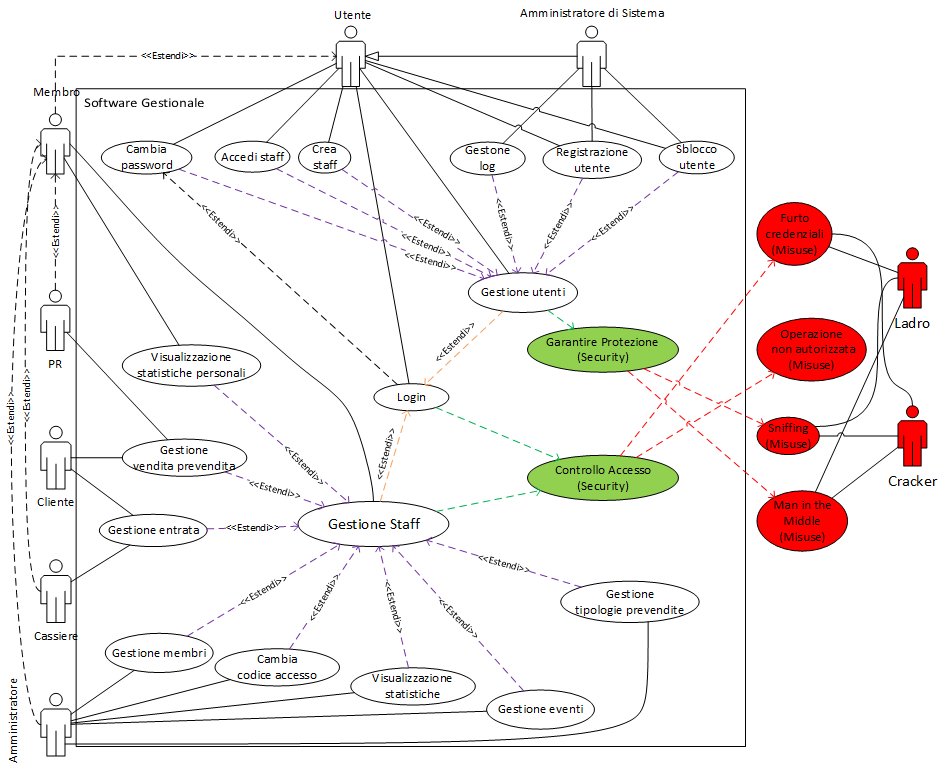
\includegraphics[scale=0.73]{security_use_cases_misuse_cases.png}

\newpage

\begin{center}
\begin{tabularx}{1\textwidth}{|X|X|X|X|}
    \hline
    \multicolumn{4}{|X|}{\textbf{Caso d’uso:} Garantire Protezione}\\
    \hline
    \multicolumn{4}{|X|}{\textbf{Descrizione:} I dati devono essere protetti, sia nella comunicazione, sia nelo stoccaggio.}\\
    
    \hline
\end{tabularx}
\end{center}

\end{document}
